\documentclass[a4paper, 14pt]{extarticle}

% Поля
%--------------------------------------
\usepackage{geometry}
\geometry{a4paper,tmargin=2cm,bmargin=2cm,lmargin=3cm,rmargin=1cm}
%--------------------------------------


%Russian-specific packages
%--------------------------------------
\usepackage[T2A]{fontenc}
\usepackage[utf8]{inputenc} 
\usepackage[english, main=russian]{babel}
%--------------------------------------

\usepackage{textcomp}

% Красная строка
%--------------------------------------
\usepackage{indentfirst}               
%--------------------------------------             


%Graphics
%--------------------------------------
\usepackage{graphicx}
\graphicspath{ {./images/} }
\usepackage{wrapfig}
%--------------------------------------

% Полуторный интервал
%--------------------------------------
\linespread{1.3}                    
%--------------------------------------

%Выравнивание и переносы
%--------------------------------------
% Избавляемся от переполнений
\sloppy
% Запрещаем разрыв страницы после первой строки абзаца
\clubpenalty=10000
% Запрещаем разрыв страницы после последней строки абзаца
\widowpenalty=10000
%--------------------------------------

%Списки
\usepackage{enumitem}

%Подписи
\usepackage{caption} 

%Гиперссылки
\usepackage{hyperref}

\hypersetup {
	unicode=true
}

%Рисунки
%--------------------------------------
\DeclareCaptionLabelSeparator*{emdash}{~--- }
\captionsetup[figure]{labelsep=emdash,font=onehalfspacing,position=bottom}
%--------------------------------------

\usepackage{tempora}
\usepackage{amsmath}
\usepackage{color}
\usepackage{listings}
\lstset{
  belowcaptionskip=1\baselineskip,
  breaklines=true,
  frame=L,
  xleftmargin=\parindent,
  language=Python,
  showstringspaces=false,
  basicstyle=\footnotesize\ttfamily,
  keywordstyle=\bfseries\color{blue},
  commentstyle=\itshape\color{purple},
  identifierstyle=\color{black},
  stringstyle=\color{red},
}

%--------------------------------------
%			НАЧАЛО ДОКУМЕНТА
%--------------------------------------

\begin{document}

%--------------------------------------
%			ТИТУЛЬНЫЙ ЛИСТ
%--------------------------------------
\begin{titlepage}
\thispagestyle{empty}
\newpage


%Шапка титульного листа
%--------------------------------------
\vspace*{-60pt}
\hspace{-65pt}
\begin{minipage}{0.3\textwidth}
\hspace*{-20pt}\centering

\includegraphics[width=\textwidth]{emblem}
\end{minipage}
\begin{minipage}{0.67\textwidth}\small \textbf{
\vspace*{-0.7ex}
\hspace*{-6pt}\centerline{Министерство науки и высшего образования Российской Федерации}
\vspace*{-0.7ex}
\centerline{Федеральное государственное бюджетное образовательное учреждение }
\vspace*{-0.7ex}
\centerline{высшего образования}
\vspace*{-0.7ex}
\centerline{<<Московский государственный технический университет}
\vspace*{-0.7ex}
\centerline{имени Н.Э. Баумана}
\vspace*{-0.7ex}
\centerline{(национальный исследовательский университет)>>}
\vspace*{-0.7ex}
\centerline{(МГТУ им. Н.Э. Баумана)}}
\end{minipage}
%--------------------------------------

%Полосы
%--------------------------------------
\vspace{-25pt}
\hspace{-35pt}\rule{\textwidth}{2.3pt}

\vspace*{-20.3pt}
\hspace{-35pt}\rule{\textwidth}{0.4pt}
%--------------------------------------

\vspace{1.5ex}
\hspace{-35pt} \noindent \small ФАКУЛЬТЕТ\hspace{80pt} <<Информатика и системы управления>>

\vspace*{-16pt}
\hspace{47pt}\rule{0.83\textwidth}{0.4pt}

\vspace{0.5ex}
\hspace{-35pt} \noindent \small КАФЕДРА\hspace{50pt} <<Прикладная Математика и информатика>>

\vspace*{-16pt}
\hspace{30pt}\rule{0.866\textwidth}{0.4pt}
  
\vspace{11em}

\begin{center}
\Large {\bf Лабораторная работа №6 } \\ 
\large {\bf по курсу <<Языки и методы программирования>>} \\ 
\large <<Программа с графическим пользовательским интерфейсом>>
\end{center}\normalsize

\vspace{8em}


\begin{flushright}
  {Студент группы ИУ9-21Б Хромов М.А.\hspace*{15pt} \\
  \vspace{2ex}
  Преподаватель Посевин Д. П.\hspace*{15pt}}
\end{flushright}

\bigskip

\vfill
 

\begin{center}
\textsl{Москва 2025}
\end{center}
\end{titlepage}
%--------------------------------------
%		КОНЕЦ ТИТУЛЬНОГО ЛИСТА
%--------------------------------------

\renewcommand{\ttdefault}{pcr}

\setlength{\tabcolsep}{3pt}
\newpage
\section{Цель}\label{Sect::task}
\par
Приобретение навыков разработки программ с графическим пользовательским интерфейсом на основе библиотеки swing.
	
 

\section{Задание}\label{Sect::task}
\par
В течение лабораторной работы нужно разработать программу, рисующую на экране одно из изображений, перечисленных в таблицах 1 – 7. Программа должна иметь графический пользовательский интерфейс, через который пользователь может задавать параметры изображения. Изображение должно перерисовываться автоматически при изменении любого параметра.
\par
Значения параметров, обозначенных в таблицах 1 – 7 латинскими буквами, представляют собой неотрицательные целые числа. Когда в описании изображения говорится о выборе цвета, подразумевается выбор из нескольких предопределённых альтернатив (например, красный, зелёный или синий).

\section {Практическая реализация}
Исходный код программы представлен в листингах~\ref{lst:code1}--~\ref{lst:code4}.
\begin{figure}[!htb]
\begin{lstlisting}[language={},caption={Main file variant 2},label={lst:code1}]
import javax.swing.*;
import javax.swing.event.ChangeEvent;
import javax.swing.event.ChangeListener;
import java.awt.*;

public class TriangleForm {
    private JPanel mainPanel;
    private JSpinner sideASpinner;
    private JSpinner sideBSpinner;
    private JSpinner sideCSpinner;
    private JTextField anglesField;
    private CanvasPanel canvasPanel;

    public TriangleForm() {
        sideASpinner.setValue(50);
        sideBSpinner.setValue(50);
        sideCSpinner.setValue(50);

        ChangeListener listener = new ChangeListener() {
            public void stateChanged(ChangeEvent e) {
                updateTriangle();
            }
        };

        sideASpinner.addChangeListener(listener);
        sideBSpinner.addChangeListener(listener);
        sideCSpinner.addChangeListener(listener);

        updateTriangle();
    }

    private void updateTriangle() {
        int a = (int) sideASpinner.getValue();
        int b = (int) sideBSpinner.getValue();
        int c = (int) sideCSpinner.getValue();

        if (canvasPanel != null) {
            canvasPanel.setSides(a, b, c);
        }

        if (a + b > c && a + c > b && b + c > a) {
            double angleA = Math.toDegrees(Math.acos((b*b + c*c - a*a) / (2.0 * b * c)));
            double angleB = Math.toDegrees(Math.acos((a*a + c*c - b*b) / (2.0 * a * c)));
            double angleC = 180 - angleA - angleB;

            anglesField.setText(String.format("A=%.1f°, B=%.1f°, C=%.1f°", angleA, angleB, angleC));
        } else {
            anglesField.setText("Error");
        }
    }

    public static void main(String[] args) {
        JFrame frame = new JFrame("Треугольник");
        frame.setContentPane(new TriangleForm().mainPanel);
        frame.setDefaultCloseOperation(JFrame.EXIT_ON_CLOSE);
        frame.pack();
        frame.setVisible(true);
    }
}


\end{lstlisting}
\end{figure}
\newpage
\begin{figure}[!htb]
\begin{lstlisting}[language={},caption={Main file variant 16},label={lst:code2}]
import javax.swing.*;
import javax.swing.event.ChangeListener;
import java.awt.*;

public class SquareForm {
    private JPanel mainPanel;
    private JPanel controlPanel;
    private JSpinner countSpinner;
    private JSpinner sizeSpinner;
    private JButton generateButton;
    private CanvasPanel canvasPanel;

    public SquareForm() {
        ChangeListener listener = e -> updateSquares();
        countSpinner.addChangeListener(listener);
        sizeSpinner.addChangeListener(listener);

        generateButton.addActionListener(e -> updateSquares());
        SwingUtilities.invokeLater(this::updateSquares);
    }

    private void updateSquares() {
        int count = (int) countSpinner.getValue();
        int size = (int) sizeSpinner.getValue();
        canvasPanel.generateSquares(count, size);
    }

    public static void main(String[] args) {
        SwingUtilities.invokeLater(() -> {
            JFrame frame = new JFrame("Разноцветные квадраты");
            SquareForm squareForm = new SquareForm();
            frame.setContentPane(squareForm.mainPanel);
            frame.setDefaultCloseOperation(JFrame.EXIT_ON_CLOSE);
            frame.pack();
            frame.setVisible(true);
        });
    }
}


\end{lstlisting}
\end{figure}
\newpage
\begin{figure}[!htb]
\begin{lstlisting}[language={},caption={Canvas variant 2},label={lst:code3}]
import javax.swing.*;
import java.awt.*;

public class CanvasPanel extends JPanel {
    private int sideA = 50, sideB = 50, sideC = 50;
    private double angleA = 60, angleB = 60, angleC = 60;
    public void setSides(int a, int b, int c) {
        if (isValidTriangle(a, b, c)) {
            this.sideA = a;
            this.sideB = b;
            this.sideC = c;
            calculateAngles();
            repaint();
        } else {
            System.out.println("Error");
        }
    }
    private void calculateAngles() {
        angleA = Math.toDegrees(Math.acos((sideB * sideB + sideC * sideC - sideA * sideA) / (2.0 * sideB * sideC)));
        angleB = Math.toDegrees(Math.acos((sideA * sideA + sideC * sideC - sideB * sideB) / (2.0 * sideA * sideC)));
        angleC = 180 - angleA - angleB;
    }

    private boolean isValidTriangle(int a, int b, int c) {
        return a + b > c && a + c > b && b + c > a;
    }

    @Override
    protected void paintComponent(Graphics g) {
        super.paintComponent(g);

        if (!isValidTriangle(sideA, sideB, sideC)) return;

        int panelWidth = getWidth();
        int panelHeight = getHeight();
        int centerX = panelWidth / 2;
        int centerY = panelHeight / 2;

        int scale = 5;

        int x1 = centerX - (sideA * scale) / 2;
        int y1 = centerY + (sideB * scale) / 2;
        int x2 = x1 + sideA * scale;
        int y2 = y1;

        double angleRad = Math.acos((sideA * sideA + sideC * sideC - sideB * sideB) / (2.0 * sideA * sideC));
        int x3 = x1 + (int) (sideC * scale * Math.cos(angleRad));
        int y3 = y1 - (int) (sideC * scale * Math.sin(angleRad));

        // Преобразование углов в RGB
        int red = (int) ((angleA / 180) * 255);
        int green = (int) ((angleB / 180) * 255);
        int blue = (int) ((angleC / 180) * 255);
        g.setColor(new Color(red, green, blue));
        g.fillPolygon(new int[]{x1, x2, x3}, new int[]{y1, y2, y3}, 3);
    }
}


\end{lstlisting}
\end{figure}
\newpage
\begin{figure}[!htb]
\begin{lstlisting}[language={},caption={Canvas variant 16},label={lst:code4}]
import javax.swing.*;
import java.awt.*;
import java.awt.event.MouseAdapter;
import java.awt.event.MouseEvent;
import java.util.ArrayList;
import java.util.Random;

public class CanvasPanel extends JPanel {
    private final ArrayList<Square> squares = new ArrayList<>();
    private final Random random = new Random();
    private static class Square {
        int x, y, size;
        Color color;

        Square(int x, int y, int size, Color color) {
            this.x = x;
            this.y = y;
            this.size = size;
            this.color = color;
        }
    }
    public CanvasPanel() {
        setBackground(Color.WHITE);
        setPreferredSize(new Dimension(500, 500));
        initMouseListener();
    }

    private void initMouseListener() {
        addMouseListener(new MouseAdapter() {
            public void mouseClicked(MouseEvent e) {
                removeSquareAt(e.getX(), e.getY());
            }
        });
    }
    public void generateSquares(int count, int size) {
        squares.clear();
        if (getWidth() < size || getHeight() < size) {
            return;
        }

        for (int i = 0; i < count; i++) {
            addRandomSquare(size);
        }
        repaint();
    }
    private void addRandomSquare(int size) {
        int width = getWidth();
        int height = getHeight();
        if (width <= size || height <= size) {
            return;
        }
        int x = random.nextInt(width - size);
        int y = random.nextInt(height - size);
        Color color = new Color(
                random.nextInt(256),
                random.nextInt(256),
                random.nextInt(256)
        );
        squares.add(new Square(x, y, size, color));
    }

    private void removeSquareAt(int x, int y) {
        squares.removeIf(sq ->
                x >= sq.x && x <= sq.x + sq.size &&
                        y >= sq.y && y <= sq.y + sq.size
        );
        repaint();
    }
    protected void paintComponent(Graphics g) {
        super.paintComponent(g);
        for (Square sq : squares) {
            g.setColor(sq.color);
            g.fillRect(sq.x, sq.y, sq.size, sq.size);
            g.setColor(Color.BLACK);
            g.drawRect(sq.x, sq.y, sq.size, sq.size);
        }
    }
}

\end{lstlisting}
\end{figure}

\newpage
\clearpage


\section{Реализация варианта 2}
\begin{center}
    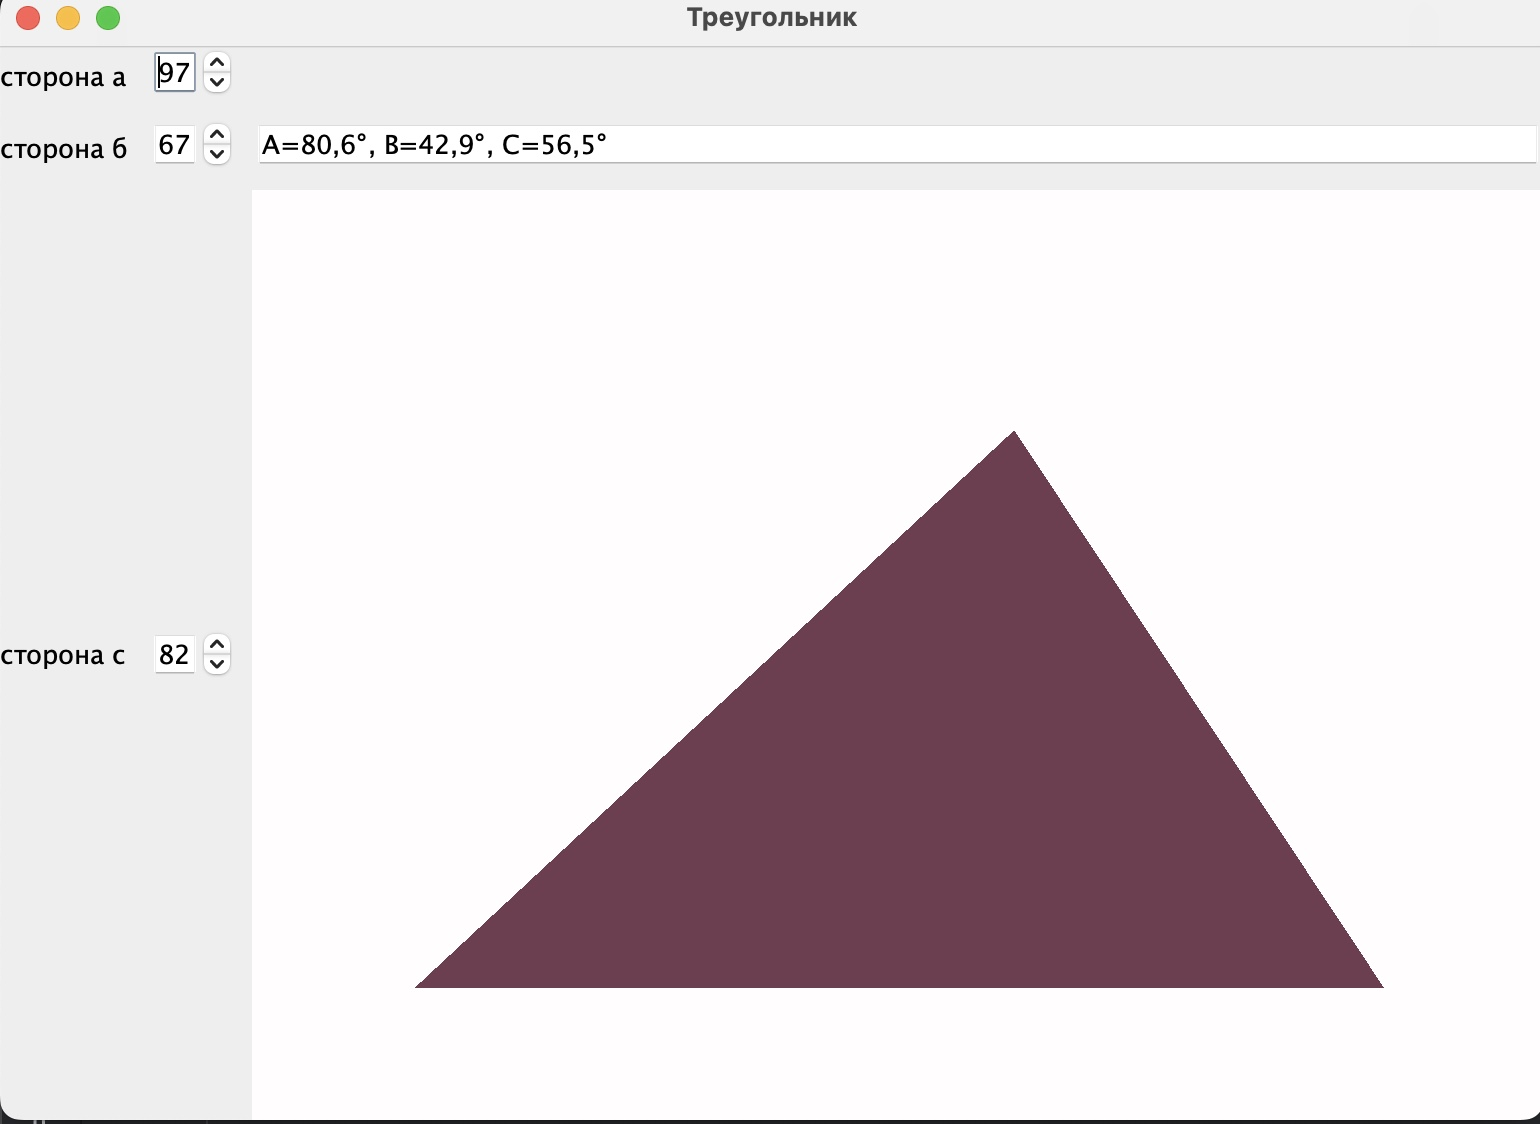
\includegraphics[width=0.8\textwidth]{фото14.jpeg}
    \captionof{figure}{Вариант 2}
\end{center}
\section{Реализация варианта 16}
\begin{center}

    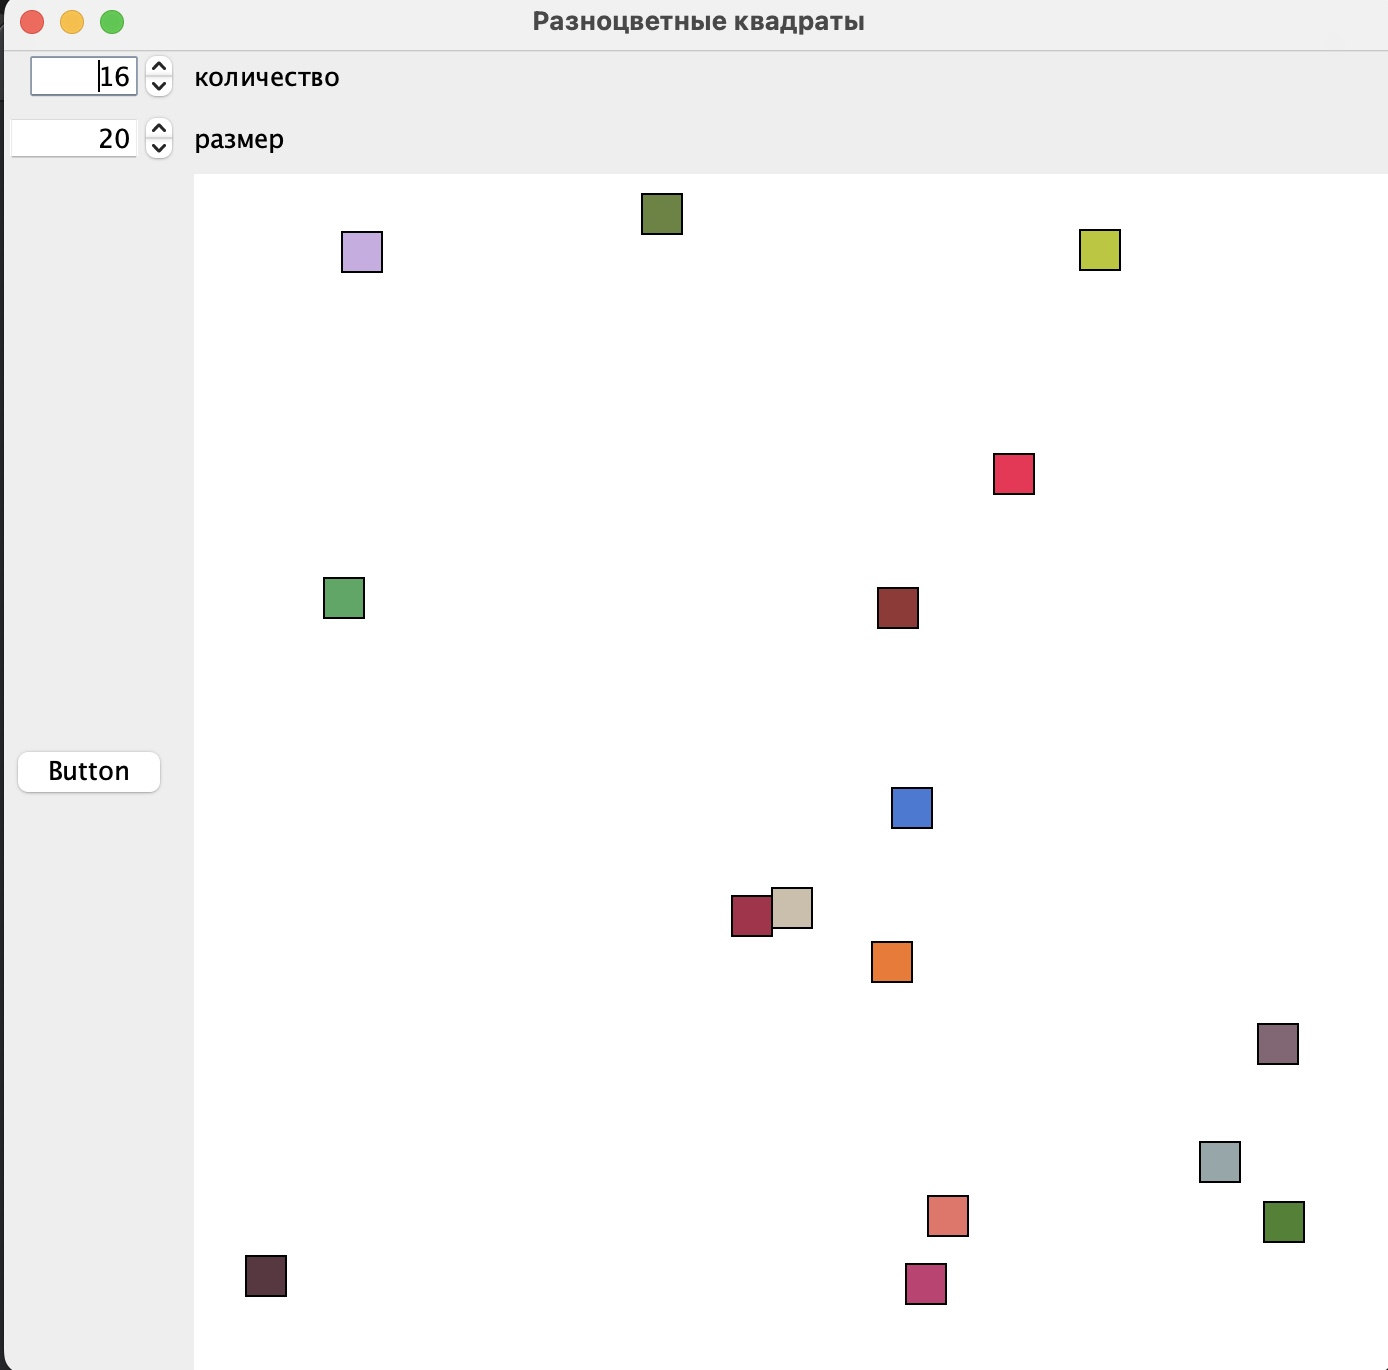
\includegraphics[width=0.8\textwidth]{фото15.jpeg}
    \captionof{figure}{вариант 16}
\end{center}

\newpage
\section{Вывод}
В ходе выполнения лабораторной работы были приобретены навыки разработки графического пользовательского интерфейса (GUI) с использованием библиотеки Swing. Были реализованы две программы: первая — для построения треугольника с заданными сторонами и вычисления его углов, вторая — для генерации разноцветных квадратов с возможностью их удаления.

Основные результаты:

Освоены базовые компоненты Swing (JFrame, JPanel, JSpinner, JButton и др.).

Изучены принципы обработки событий и динамического обновления интерфейса.

Получен опыт работы с графикой (отрисовка фигур, изменение цветов).

Программы успешно выполняют поставленные задачи, демонстрируя гибкость и удобство Swing для создания интерактивных приложений.

\end{document}